\section{Introduction} \label{sec:intro}

The smart grid is a distributed energy network composed of intelligent
nodes (or agents) that can either operate autonomously or communicate and share energy \cite{weiss1999multiagent}.
The purpose of a smart grid is to efficiently deliver energy to consumers as well as store and convert
energy produced, e.g., according to prices, supply and demand. 

A microgrid is a networked group of distributed energy sources with the goal of
generating, converting and storing energy. 
While the main power stations are highly connected, micro-grids with local power generation, storage
and conversion capabilities, act locally or share power with a few neighboring micro-grid nodes \cite{farhangi2010path}.
This scenario is being envisaged as an important alternative to the conventional scheme with
large power stations transmitting energy over long distances.

 In order to take full advantage of the modularity and flexibility of micro-grid technologies, smart
control mechanisms are required to manage and coordinate these distributed energy systems so as to
minimize the costs of energy production, conversion and storage, without jeopardizing grid stability.

The implementation of such smart controls is by no means easy for the following reasons:
\begin{inparaenum}[\bfseries (i)]
\item Small scale energy production and storage is intrinsically
         related to intermittency of wind/solar energy and to variability in the load profile.
          So an important challenge is to increase resilience and reliability under stochastic supply and
                 demand.
\item Micro-grids can operate in two different modes: (a) when they are connected to the
main power grid, and (b) in the isolated or island mode. Moreover, they can share energy with
other microgrids that require energy. Thus, one needs to make
dynamic decisions on (a) when to operate in the connected (to the power grid) or isolated modes, 
(b) when to share energy with other microgrids and when to store energy for future use, and (c) 
which form to store energy given that storage management itself
involves heterogeneous storage technologies with different
operating characteristics.
%\item Each microgrid has access to only its local (and not global) state information. 
%While microgrids can exchange information with one another, there are problems with frequent communication
%between microgrids due to (a) privacy issues and (b) risk of cyber attacks.
%Important challenges here include (a) optimizing global grid performance with limited communications,
%(b) voltage and frequency control for grid stabilization.
%\item Decision making in microgrids needs to take place on different timescales. On the slower
%timescale of say hours, one needs to make decisions on energy generation, conversion and storage,
%while on the faster timescale of minutes to seconds, one needs to make decisions related to dynamic
%demand response as well as ensuing grid stability, i.e., of frequency and voltage regulation.
\end{inparaenum}


In this paper, we address two  problems. First,  energy sharing among the microgrids under stochastic supply and demand (mentioned above as (i) and (ii)) along with the optimal battery scheduling of a microgrid from the supply-side management (SSM) perspective. Second is from the demand-side management (DSM) perspective, which is efficiently scheduling the time adjustable demand from smart appliances in the smart home environment, called as an ADL (activity of daily living) demand along with the normal demand.  Our goal here is to reduce the energy demand and supply deficit in the long-run. We address this learning and scheduling problem by modeling them as a Markov decision process (MDP) \cite{puterman2014markov, vol2}. 

%\begin{enumerate}[label={\bf\Roman*}]
\subsection{Supply-side management problem} \label{subsec:ssm}
 Supply-side management (SSM)\cite{} deals with developing techniques to  generate, transmit and distribute energy efficiently at supply-side. Cooperative energy exchange among microgrids is a popular technique in SSM for efficient energy distribution.  Local energy sharing/exchange between microgrids has the
following advantages:
(a) it can significantly reduce power wastage that would
otherwise result over long-distance transmission lines, and (b) it
helps satisfy demand and reduce reliance on the main grid. 
%Most importantly, energy exchange between microgrids needs to take place {\em with limited communication/information exchange}.
 Figure~\ref{gridmodel} shows a cooperative energy exchange model with multiple microgrids
(on the distribution side of the network) that can cater to their individual
local loads. Each microgrid controls its local sub-network through its controller (labelled
$\mbox{C}_1$, $\mbox{C}_2$ etc.) that mainly has access to its local state information.


\begin{figure}[thpb]
      \centering
      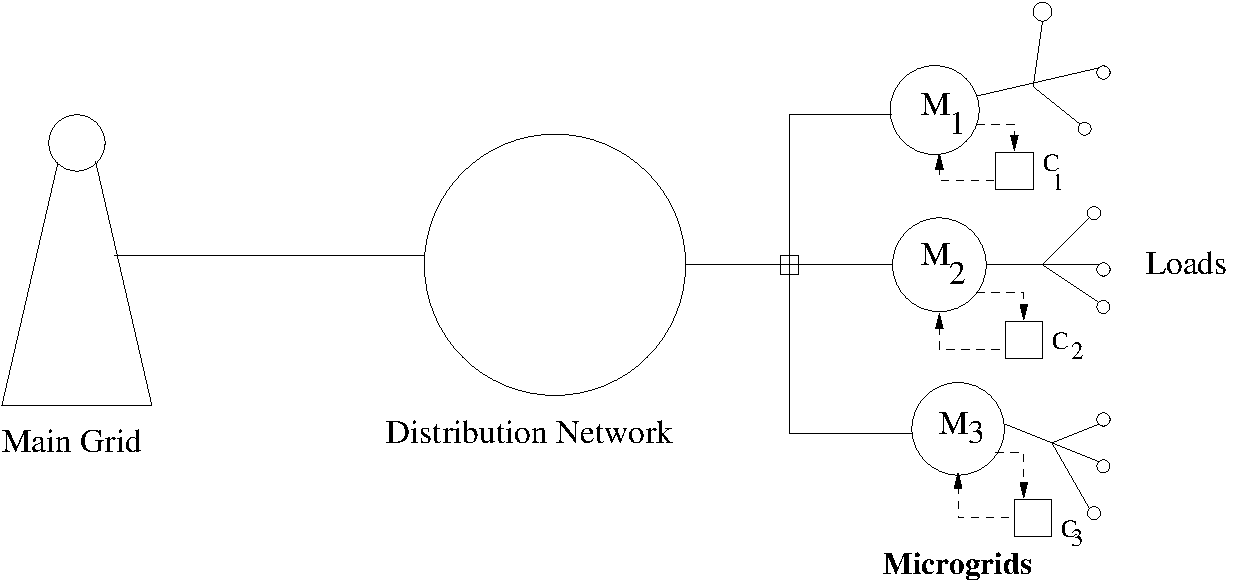
\includegraphics[scale=0.4]{powergrid2.pdf}
      \caption{Cooperative Energy Exchange Model}
      \label{gridmodel}
\end{figure}

 In classical power grids, system level optimization is done based on a centralized
objective function, where as 
microgrid network has heterogeneous nature right from the manner in which electricity
is generated such as from wind turbines, solar farms and diesel generators
to energy storage devices such as batteries and capacitors.
 Because of this heterogeneity and the fact that energy can be shared between microgrids depending
on requirements, one needs to consider asynchronous distributed techniques 
%such as multi-agent reinforcement learning or game theory
 to control and optimize a smart grid system
with a microgrid distribution network.



\textbf{Related work :} \cite{saad2012game} provides a survey on game theoretic approaches for microgrids where both cooperative energy sharing models as well as non-cooperative game models for distributed control of microgrids are examined when the system model is known. Since  models for energy dynamics are very unreliable \cite{zamora2010controls}, one has to use model-free algorithms to address these problems.  Because of their model-free nature, reinforcement learning \cite{sutton1998reinforcement} approaches that are primarily data-driven control techniques are playing a significant role in these problems.

In \cite{zifadistributed}, distributed reinforcement learning algorithm for coordinated energy sharing and voltage restoration in a islanded DC microgrid is proposed. In \cite{leo2014reinforcement}, reinforcement learning algorithm for optimal battery scheduling under the dynamic load environment and sloar power is proposed with the goal of  reducing  energy consumption from the main grid. In this paper, we  consider the coordinated energy sharing among the grid connected microgrids with optimal battery scheduling problem when stochastic supply and adjustable stochastic demand is available.



 





%make use of renewable and non-renewable energy at the supply side. 
%****************** NEEDS TO BE CHANGED


%In \cite{PHarsha}, authors consider the problem of optimal energy storage management problem under dynamic cost setup. They consider a renewable generator that is equipped with a limited storage battery and capable of meeting the some local demands. It also has connection from the main grid. The decision to be taken at every instant is the number of power units to be stored in the battery. They allow this to be negative as power can be drawn from the battery. They formulate this problem as a Markov Decision Process under long run average cost. The objective is to minimize the long run average cost of power bought from the main grid.
%
%The assumption made in this paper is that demand at all times can be met. This is facilitated by allowing the main grid as many units of power as asked by the renewable generator. In our work, we extend this MDP model to put additional constraint on the maximum number of power units that a main grid can provide. Another notable contribution is that we extend this setup to the multiple microgrids. Here, we allow the microgrids to share the power among themselves.  

%In \cite{reddy2011learned}, they consider the problem of maximizing the profits among the broker agents. These agents buy the power from the producers and sell it to the customers. They apply Reinforcement Learning (RL) algorithms to solve this problem to show that learning policies perform better than the traditional non-learning strategies.

%In \cite{goodmdp}, authors propose an MDP for solving the problem of minimizing the demand and supply deficit  
%and apply dynamic optimization methods. But when the model information (the renewable energy generation in this case) is not known, we cannot apply these techniques.

%Demand side management (DSM) (\cite{logenthiran2011multi, wang2010demand,dsm1,dsm2,dsm3,dsm4}) deals with techniques developed to efficiently use the power by bringing the customers into the play. The main idea is to reduce the consumption of power during peak time and shifting it during the other times. This is done by dynamically changing the price of power and sharing this information with the customers. 

%*********************
\subsection{Demand-side management problem}\label{subsec:dsm}
 Load shifting is a popular technique used in demand-side management (DSM) \cite{DTU2010}. It involves moving the consumption of load to different times within an hour, or within in a day, or even within a week. It doesn't lead to reduction in net quantity of energy consumed, but simply involves changing the time when the energy is consumed. Advantage due to load shifting for the customer is reduction in the energy consumption cost, and the advantage for the smart grid is in managing the peak load consumption. Hence load shifting is beneficial for both the consumers and the smart grid.

With the increased use of the smart appliances and smart home environments, the concept of load shifting is becoming increasingly handy for the smart grid as the demand from smart appliances is time adjustable in general. One or more of these smart appliances collectively achieve some activity in the smart home environment, called as an ADL (activity of daily living). It's possible to monitor and identify the ADLs in the smart home environments \cite{I2014, GPG2016}. When an ADL is active, the smart appliances associated with that ADL are switched on to perform the activity defined by the ADL thus adding load on the smart grid. With the help of the smart home technology, it's possible to find the amount of load each ADL puts on the grid, and also the allowed time window during which the ADL would perform the activity (e.g., washing machine running for an hour to clean the cloths anytime between 3PM to 6PM). If the time window for the ADL lets the smart grid have more than one possible way of scheduling the load, it's considered as flexible ADL. On the other hand, if the time window for the ADL lets the smart grid have exactly one possible way of scheduling the load, it's considered as non-flexible ADL (e.g., washing machine running for an hour to clean the cloths anytime between 3PM to 4PM, is not flexible since there is only one option of switching on the washing machine at 3PM). Thus the demand from the flexible ADLs need not be met at a fixed time period, instead could be met at any time period within a flexible time window. With the help of the advanced metering infrastructure (AMI) \cite{RAFK2014} that provides a two-way communication between the utility and customers, it's possible to take the decision of when to schedule the ADL demand at the smart grid and convey the same to the customer's smart meter.    

There is other regular demand that needs to be met at fixed time periods, apart from the zero or more ADL related demand associated with any customer. This regular demand along with the zero or more non-flexible ADL demand of a smart home is considered to be non-ADL demand for the rest of the paper. Similarly, the demand due to zero or more flexible ADLs of the smart home is considered to be ADL demand.
 
There is prior art around scheduling the ADL-demand using the load shifting technique for handling the peak load scenarios \cite{CL2014}. However, they precisely know the supply profile while doing such a scheduling of the ADL-demand. In this paper, we propose scheduling of ADL-demand using the load shifting technique with uncertainty in the supply profile generated (e.g., renewable energy sources like solar or wind being the primary sources of power generation).
%\end{enumerate}

%Research on smartgrids can be classified into two areas -  Demand-side management and Supply-side management.

 

%In \cite{reddy2011learned}, Reinforcement Learning (RL) is used in smart grids for pricing mechanism so as to improve the profits of broker agents who procure energy from power generation sources and sell it to consumers.  
\textbf{Our contributions :}
\begin{inparaenum}[\bfseries (i)]
We summarize our contributions as follows :\\
\item To the best of out knowledge, we are the first one to integrate both the Demand-side and Supply-side management problems  in a single Markov decision process framework. We used reinforcement learning algorithms which do not require knowledge of the underlying model to address these problems. Our algorithms are easy to implement and also scalable.\\
\item The Optimal scheduling of ADL demand at microgrid level, where both the demand and power generation is stochastic is first time introduced through this work. \\    
\end{inparaenum}
%\section*{Organization of the Paper}	


The rest of the paper is organized as follows. The next section describes the important problems associated with the microgrids and solution techniques to solve them. Section III presents the results of experiments of our algorithms. Section IV provides the concluding remarks and Section V discusses the future research directions.